\subsubsection{Linhas de distribuição (condutores)}

\begin{enumerate}
	\item A bitola mínima dos circuitos terminais deverá ser de acordo as estabelecidas na seção \ref{lighting - generalidades} item \ref{lighting: bitola minima} e seção \ref{section: socket-general} itens \ref{socket: bitola minima} e \ref{socket: bitola minima ar} ;

	\item Dimensionar a bitola do condutor conforme a capacidade de condução de corrente e a queda de tensão admissível, considerando os fatores de correção de temperatura de agrupamento de cabos. 

	\item Limitar a queda de tensão, entre a origem da instalação e qualquer ponto de utilização, a valores compatíveis com a norma NBR 5410. 

	\item Dimensionar os alimentadores de modo a transmitir potência suficiente aos circuitos alimentadores, bem como para atender a futuros aumentos de carga. 

	\item Dimensionar, especificar e identificar os circuitos de acordo com a NBR-5410.
	
\end{enumerate}

\paragraph{O que evitar}

TEXTO nesta subseção precisa ser reeescrito (lançado apenas a título de não esquecer o que queremos)

\begin{enumerate}
	\item \textcolor{orange}{Na imagem XXXXX veja que existe uma eletrocalha em verde (indicada pela linha de chamada com o símbolo 'A'), agora observe que a dimensão da eletrocalha não está indicada onde temos a distribuição com o símbolo 'A'(imagem XXXXX) e a dimensão da mesma não pode ser a mesma que encontra-se indicada na legenda conforme visto na imagem XXXX, pois na imagem XXXXX a representação da dimensão da eletrocalha existente 300x100mm não é a mesma da eletrocalha indicada na cor verde, logo não é possível afirmar qual é a real dimensão da eletrocalha.
	}
	
	\item \textcolor{orange}{Observe a imagem XXXX, poderíamos deduzir que a bitola de todos os cabos indicados é a mesma, entretanto não existe indicação em nota da real bitola dos cabos não cotados, tornando impossível deduzir a bitola dos cabos.
	}
	
	\item \textcolor{orange}{Existindo cabos com diferentes bitolas as mesmas devem ser representadas em planta. Não será aceito que a indicação das bitolas conste apenas no quadro de cargas.
	}
\end{enumerate}



\begin{figure}[H]
	\centering
	\begin{subfigure}[b]{0.45\textwidth}
		\centering
		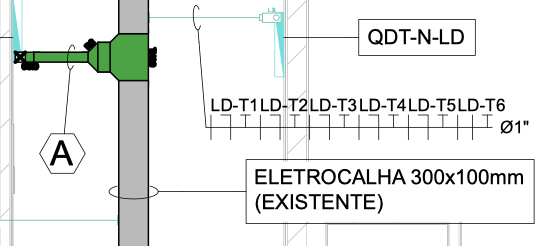
\includegraphics[width=\textwidth]{Figures/6. Distribution/avoid1a.png}
		\caption{image a}
		\label{fig: style 1 avoid a}
	\end{subfigure}
	\hfill
	\begin{subfigure}[b]{0.45\textwidth}
		\centering
		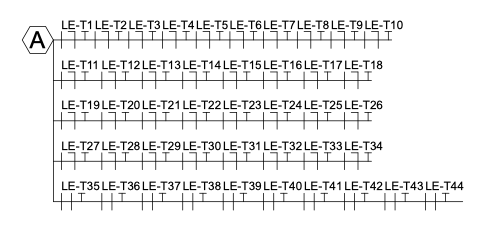
\includegraphics[width=\textwidth]{Figures/6. Distribution/avoid1b.png}
		\caption{image b}
		\label{fig: style 1 avoid b}
	\end{subfigure}
	\hfill
	\begin{subfigure}[b]{0.9\textwidth}
		\centering
		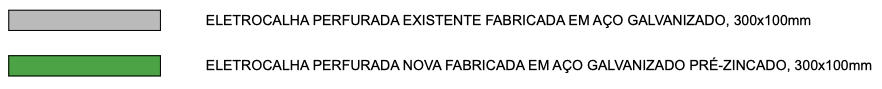
\includegraphics[width=\textwidth]{Figures/6. Distribution/avoid1c.png}
		\caption{image c}
		\label{fig: style 1 avoid c}
	\end{subfigure}
	\caption{Three images}
	\label{fig: style 1 avoids}
\end{figure}
